\documentclass[11pt]{article}

\usepackage[margin=0.5in]{geometry}
\usepackage{fancyhdr}
\usepackage{graphicx}
\pagestyle{fancy}
\usepackage{amsmath}
\usepackage{amssymb}

\lhead{CSN-212 Assignment \#2}
\chead{Gaurav Kumar Gupta, ECE IV, 13116027}
\rhead{January 13, 2017}


\begin{document}

\begin{section}{Data Structures}
Data can be stored and organized in a system for efficient use in particular ways or structures known as data structures. Here are a few types of data structures:
\begin{enumerate}
\item Array: It is a collection of elements which is assigned a contiguous block of memory. It has a common variable name and index.
\item Stack: It's a linear data structure where the order of operations is either FILO or LIFO.
\item Queue: It's also a linear data structure where the order of operations is FIFO.
\item Linked List: A group of nodes representing a sequence constitute a linked list. Each node comprises of data item and a pointer to the next node in the sequence. The first node is marked by a head pointer while the end node points to null.Linked Lists can also be circular or(and) doubly linked.
\item Binary Tree: It comprises of a set of nodes having data and references to their children nodes. In this hierarchical structure no node points to the root. a binary tree maybe a AVL, Binary Search Tree, Red Black Tree etc. 
\begin{figure}[ht!]
\centering
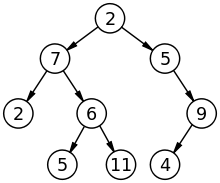
\includegraphics[width=20mm,scale=0.4]{bt.png}
\end{figure}
\item B-Tree: It's a self balancing binary tree in which each node can have more than 2 children, mainly used for information retrieval and storage.
\item Binary Heap: It's a complete binary tree which is either min or max heap. In a Min Binary Heap, the key at root must be minimum among all keys present in Binary Heap. The same property must be recursively true for all nodes in Binary Tree.
\item Graph: It’s a collection of a set of vertices V and a set of edges E. Each edge E is a pair (v, w) where v and w are elements of V.
\begin{figure}[ht!]
\centering
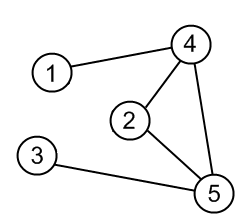
\includegraphics[width=20mm,scale=0.4]{graph.png}
\end{figure}
\item Hashes: A hash is a dictionary like set of unique keys and values.An item and the slot(or index) where it belongs in the hashmap and hashtable is mapped through a hash function.
\end{enumerate}
\end{section}
\begin{section}{About Me}
\paragraph{}I am Gaurav Kumar Gupta. I am from Electronics and Communication Department. My research interests lie in Data Science, Machine Learning and Social Network Analysis. I interned in Adobe Research, Bangalore in my junior year. I worked on a project titled 'Personalized Content Scoring Model for Behance'.The objective of the project was to provide users with personalized suggestions for artworks and designs on Behance, an online platform to showcase creative work. I also intend to join Adobe after I graduate after receiving a job offer. I am doing my B.Tech Project under the guidance of Prof. P.M. Pradhan, Dept. Of Electronics and Comm. Engineering.The project titled 'Sleep Scheduling in Wireless Sensor Networks Using Reinforcement Learning',aims to develop a a reinforcement learning-based sleep scheduling for coverage algorithm for sustainable time-slotted operation in rechargeable sensor networks I feel that I have a strong acumen for research. I plan to go for M.S. next year either in Europe or US. My other projects include an 'Android Based Application for Augmented Reality', aimed at developing mobile augmented reality and image recognition platform enabling advertisers to reach consumers
via outdoor ads, billboards, magazine, newspaper etc., and a face recognition application that sends a notification to a person's mobile telling them who is at the door. 

\end{section}
\end{document}